\documentclass[../main.tex]{subfiles}

\begin{document}

\chapter{“Xin lỗi chịu hổng nổi” hay là kiểu chơi cù cum ngôn ngữ xuất tinh trong}

\begin{metadata}

\begin{flushright}19.7.2008\end{flushright}

Liêu Thái



\end{metadata}

\begin{multicols}{2}

\begin{figure}
	\centering
	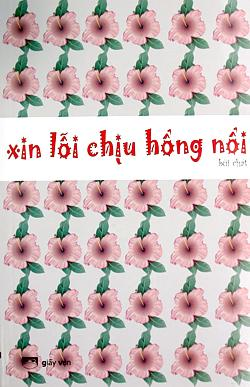
\includegraphics[width=\textwidth]{../img/tho190708.jpg}
	\caption{
\textit{Xin lỗi chịu hổng nổi}, thơ nghĩa địa Bùi Chát, Nhà xuất bản Giấy Vụn, Sài Gòn, 12/2007}
\end{figure}
Người bị bệnh xuất tinh trong là kẻ có khả năng tình dục ghê gớm nhưng khả năng thụ thai thì cũng yếu gớm ghê, vì hắn có khả năng làm cho người tình của hắn sướng đến vỡ óc nhưng bản thân hắn thì cứ làng nhàng không buồn không vui, dịch chuyển cơ bắp như một thứ trách nhiệm. (Khổ nỗi trách nhiệm mà hắn chú ý duy nhất lại là tự làm cho mình sướng, nhưng càng làm vậy, hắn càng đau khổ trong tiếng rên của người khác!). Trong thú chơi ngôn ngữ, đặc biệt là ngôn ngữ thơ, kẻ nào xung năng quá lớn, ý niệm sung mãn, tư duy lạnh và có khả năng nuốt từ rác đến cứt ngôn ngữ mà vẫn đẻ được trứng thì đương nhiên cuộc đời hắn sẽ phải đón nhận một bi kịch nào đó trong sự sung sướng của kẻ khác, chẳng khác gì mình phải quằn quại nuốt rác trong sự đe doạ tù tội để thay thế con gà đẻ trứng! \textit{\textbf{Xin lỗi chịu hổng nổi}} của Bùi Chát là trường hợp mang nghiệp luỵ này. Thử xẻ một vài lát trên cấu trúc ngôn ngữ, mổ một vài nhát lên kỹ thuật dụng ngôn và săm soi (chứ không phải soi mói) lại toàn bộ cái thân thể loã lồ của những cô gái điếm hết hạn được chơi cù cum tréo ngoe, ngược trục một cách vuông vức trong phương pháp chơi đùa chữ nghĩa của anh ta chẳng hạn! 
\begin{blockquote}


\textit{Anh sợ những cột đèn đổ xuống} 
\textit{Rồi dây điện cuốn lấy chúng ta} 
\textit{Bóp chết mọi hy vọng} 
\textit{Nên anh dìu em đi xa} 
\textit{Í a} 

\textit{Đi đi chúng ta đến công viên lê văn tám} 
\textit{Nơi anh sẽ hôn em đắm đuối} 
\textit{Ôi môi em như mật đắng} 
\textit{Như móng sắc thương đau} 
\textit{Như móng sắc thương đau} 
\textit{Đi đi anh đưa em vào quán rượu} 

\textit{Được chứ!} 

Nguyên liệu: “Dạ khúc” của Thanh Tâm Tuyền 

(“Tìm mọi cách để rủ người yêu đi nhậu” – tr. 94) 

\end{blockquote}


Tôi từng viết về Bùi Chát vào năm 2003\footnote{\url{http://www.talawas.org/talaDB/http://cafe.damau.org/?p=318}} khi anh cho ra mắt tập thơ \textit{Xáo chộn chong ngày}\footnote{\url{http://www.talawas.org/talaDB/http://www.talachu.org/tho.php?bai=19}}\textit{ }(nxb Giấy Vụn – La Hán Phòng). Ngay lúc đó người viết cũng đã nhận ra rằng tác giả thơ này có tạng ngôn ngữ cong, cấu trúc và tốc độ biến thể ngôn từ nhanh một cách rất… lười biếng và có dấu hiệu xuất tinh trong trên phương diện diễn từ. Mãi đến năm 2008, đúng năm năm sau, cầm lại tập thơ cũ, đối chiếu, so sánh với \textit{Xin lỗi chịu hổng nổi}, có thể nói là tính cù cum, tréo ngoe, ngược trục trong ngôn ngữ thơ anh đã biểu hiện rõ nét, mạnh mẽ hơn trước đây nhiều lần. Nó tạo cho người đọc thú vui nhiều hơn là phải vắt óc ra mà suy nghĩ về một triết lý hay cố gắng dán một mỹ cảm nào đấy tưởng chừng hợp lý cho thơ, nhưng nó cũng không đến nỗi dễ dãi, đơn giản để không cần suy tư, thậm chí là suy tư với cường độ cao mới có thể hiểu được hành động bỡn cợt trong thơ của tác giả này muốn nói lên điều gì. Và vấn đề được đặt ra là: vì sao anh ta lại chọn thái độ dễ dãi, bỡn cợt và nhảm nhí? Vì sao mức độ nhảm nhí mỗi lúc một tăng cao? Anh ta chọn thái độ như vậy một cách bền bỉ nhằm nói lên điều gì? 
\begin{blockquote}


\textit{tôi hỏi đất: - đất sống với đất như thế nào?} 
\textit{- chúng tôi tôn cao nhau [heo]} 

\textit{tôi hỏi nước: - nước sống với nước như thế nào?} 
\textit{- chúng tôi làm đầy nhau [heo]} 

\textit{tôi hỏi cỏ: - cỏ sống với cỏ như thế nào?} 
\textit{- chúng tôi đan vào nhau [heo]} 
\textit{làm nên những chưn trời} 
\textit{chơi &amp; bời} 

\textit{tôi hỏi thỉnh: }
\textit{- thỉnh sống với thỉnh như thế nào?} 
\textit{[ối dào!]} 
\textit{tôi hỏi người:} 
\textit{- thỉnh sống với người như thế nào?} 
\textit{[ối dào!]} 
\textit{tôi hỏi người:} 
\textit{- thỉnh sống với người như thế nào?} 
\textit{[ối dào!]} 

Nguyên liệu: “Hỏi” của Hữu Thỉnh 

(“Hỏi đáp có thưởng” – tr. 25) 

\end{blockquote}


Thật ra, để trả lời những câu hỏi trên có lẽ chính tác giả mới có thể thoả đáng trong chừng mực nào đó. Phần lớn chúng ta ưa phán quyết một cách chính xác những gì thuộc về mù mờ, đoán mò. Nhưng dù sao đi nữa, đã là người Việt, sống ở xứ sở tranh tối tranh sáng này mà không một lần đoán mò thì e rằng chẳng còn tí tính Việt nào cả! Và làm thơ, trong một ý nghĩa nào đó cũng cách gián tiếp đoán mò định mệnh văn học và định mệnh dân tộc, như thầy bói xem voi trong câu chuyện ngụ ngôn Ấn Độ chẳng hạn! Và ở đây, câu chuyện ngụ ngôn cần được hiểu như nó vốn vậy! 
\begin{blockquote}


\textit{Ông Lê nin ở nước Nga} 
\textit{Cớ sao ông đứng vườn hoa nước mình} 
\textit{Một tay chỉ một tay khuỳnh} 
\textit{Đằng sau một lũ rập rình ăn theo} 

\textit{Làm bọn tôi phải đói meo} 
\textit{Nói cho dễ hiểu là seo bây giờ} 

\textit{- chờ!} 

Nguyên liệu: Ca dao hiện đại &amp; bài thơ của bạn Võ Hạnh Thắm, học sinh lớp 6 Hà Nội đã giành giải Nhất về thơ cuộc thi viết vẽ về “Cách mạng tháng Mười và đất nước của Lê nin vĩ đại” do báo Đội tổ chức cách đây hơn 20 năm, nhân kỷ niệm 70 năm Cách mạng tháng Mười Nga vĩ đại. Bạn Thắm có viết: \textit{“Ông Lê nin ở nước Nga. Mà sao em thấy rất là Việt Nam…”} (Thông tin mới bổ sung từ báo \textit{Thiếu Niên Tiền Phong}, 13/11/2007). 
\textit{}
(“Chờ” - tr. 39) 

\end{blockquote}


Trung bình mỗi năm, tại Việt Nam, số lượng đầu sách (không kể đến sách giáo khoa) xuất bản không nhỏ và có dung lượng tri thức na ná giống nhau cũng không nhỏ tí nào. Giả sử nếu một người chịu khó đọc khoảng chừng 50 cuốn sách được xuất bản trong một năm/ dưới sự cho phép của chính quyền (hay còn gọi là in ấn hợp pháp) thì có mù mắt cũng nhận ra được hàng tá những ý na ná nhau trong đó. Hoặc vì lí do sống cùng thời, hoặc vì không biết nhau, cùng chung “tư tưởng lớn” – đại để là vậy! Hoặc vì một lý do lớn nhất, mà đây cũng là nguyên nhân của mọi đui què mẻ sứt trong cái sáng tạo ở xứ này – cùng sáng tạo dưới ánh sáng của chủ nghĩa xã hội (hoặc chủ nghĩa cộng sản hoặc xã hội chủ nghĩa… Ba chủ nghĩa này về mặt nội hàm hoàn toàn khác nhau nhưng đã được đọc và hiểu như nhau từ lâu rồi, một kiểu đánh tráo khái niệm ấy mà!). Đó là chưa nói đến thơ. Thử đọc một số tập thơ của những năm 1980, sẽ thấy có nét gì đó hao hao thơ thời 1930 – 1945. Đọc lại thơ những năm 2000, người đọc vẫn còn nhận thấy rúc rích đâu đó cái tinh thần lạc quan rởm của các cô cậu sinh viên, càng đọc càng thấy na ná nhau, chẳng đâu vào đâu! 
\begin{blockquote}


\textit{Con ở* miền nam lăng** ra thăm bác} 
\textit{Con thấy lăng ông còn thua lăng bác} 
\textit{Từ đó con trở nên chững chạc} 

\textit{---------------} 
\small{\textit{* Con ở: con sen, người giúp việc..}} 
\small{\textit{** Lăng: âm miền nam của lăn}} 

Nguyên liệu: “Viếng lăng Bác” của Viễn Phương 

(“Xin cảm ơn” – tr. 10) 

\end{blockquote}


Sự ra đời của một nhóm thơ, nhiều nhóm thơ trên căn bản đập phá những thứ nên thay đổi trên đây đã mang lại ít nhiều sinh khí cho thơ Việt. Cái nó mang lại nhiều nhất trong giai đoạn đầu có lẽ là sự lặp lại một cách minh bạch mang tính giễu nhại những cái được mệnh danh mẫu - mực - liên - văn - bản và phác hoạ một cái nhìn mới, một “biểu đồ” mới cho thơ (dù rằng hành động bứt phá sáng tạo của họ vẫn còn đang ở dạng xây nền móng và gặp không ít trở ngại…). 
\begin{blockquote}


\textit{Vườn nay người khác đã rào} 
\textit{Khóm mai thay chỗ khóm đào ngày xưa} 
\textit{Em ngồi nhặt áo giữa trưa} 
\textit{Đâu rồi môi hát vu vơ một mình..} 
\textit{Em ngồi giặt áo lặng thinh} 
\textit{Vò cho sạch những vết tình còn vương} 
\textit{Giũ cho rơi bớt giọt buồn} 
\textit{Phơi cho khô hết nhớ thương xa vời..} 

\textit{Thơ Kiều có vận vào đời em chăng?} 
\textit{Tình so chưa đủ ngũ âm} 
\textit{Áo chồng con đã nặng oằn dây phơi} 
\textit{Áo ca dao gió cuốn rồi} 
\textit{Cầu ca dao trả cho người khác qua} 
\textit{Tóc mai rũ bóng hiên nhà} 
\textit{Chuyện xưa dù nhắc cũng là chuyện xưa} 

\textit{Em ngồi giặt bướm giữa trưa} 
\textit{Rát bàn tay vẫn vò chưa sạch lồn} 

\textit{Có thể chỉ là tin đồn} 

Nguyên liệu: “Lỗi hẹn cùng ca dao” của Thanh Nguyên 

(“Lỗi hẹn cùng ca dao búa liềm” – tr. 88) 

\end{blockquote}


Kỹ thuật bẻ chữ, dán đuôi vào “tác phẩm nguồn”, nguyên liệu (có lẽ nói rằng thuật ngữ “tác phẩm nguồn”, “nguyên liệu” ra đời sau sự xuất hiện \textit{Xáo chộn chong ngày} là hoàn toàn chính xác!) khiến những bài thơ xuất hiện lần này có nét quái [vật] hơn, kì dị [hợm] hơn, tạo ra nhiều khôi hài, bất ngờ khiến độc giả có thể bật cười trước những cái từng được xem là nghiêm túc, chuẩn mực. Kỹ thuật dán đuôi vào tác phẩm nguồn còn tạo ra hiệu ứng đường vòng trong ngôn ngữ, tính đa chiều được kích hoạt theo quĩ đạo xoắn ốc, mô hình nở. Dường như đây cũng là linh cảm, mối tương quan giữa thi sĩ và xu hướng mất trật tự của vũ trụ? 
\begin{blockquote}


\textit{Sao anh lại rình }
\textit{Trộm xem em tắm} 
\textit{Da của em ngần trắng} 
\textit{Da cha mẹ cho em} 
\textit{Tay của em lấm lem} 
\textit{Tay của than của bụi} 
\textit{Tay của rừng, của núi} 
\textit{Tay của đất, của nương} 
\textit{Em tắm xong lại sạch} 
\textit{Vẫn ngát thơm hoa rừng} 
\textit{Da của em trắng ngần} 
\textit{Là của anh tất cả} 
\textit{Không phải người xa lạ} 
\textit{Việc gì mà trộm xem} 
\textit{Em tắm giữa suối Mường} 
\textit{Tắm trong mối yêu thương} 
\textit{Có anh đang đứng giữ} 
\textit{Chớ để Tây đến Mường} 

\textit{Bằng không em chán chường} 
\textit{Sẽ cóc thèm đi tắm} 
\textit{Trên người em mùi khắm} 
\textit{Sẽ bay toả khắp nơi} 
\textit{Lúc đó mà thèm chơi} 
\textit{Cũng không sao chịu được} 
\textit{Bây giờ em đánh cược} 
\textit{Sẽ không hề nói điêu} 
\textit{Nếu mà anh có liều} 
\textit{Thì để Tây nó đến} 
\textit{Em thì chiều tới bến} 
\textit{Khi mô cũng sẵn sàng} 
\textit{Nghe có vẻ phũ phàng} 
\textit{Không tin thời cứ thử} 
\textit{Em ngu gì tự tử} 
\textit{Chỉ không tắm vậy thôi} 
\textit{Rồi cứ để mà coi} 
\textit{…} 

\textit{Em không thèm nói nữa!} 

Nguyên liệu: “Em tắm” của Bạc Văn Ùi 

(“Uy hiếp người yêu” – tr. 75) 

\end{blockquote}


Một khi cái biểu tượng, thiết chế bị/được qui giản vào một chủ nghĩa, một hệ tư tưởng, một sự ràng buộc có tính chế tài và ý nghĩa về tự do bị đồng nhất với một sự cho phép, một giới hạn, một đồng thuận đại tự sự nào đấy thì khái niệm sáng tạo chỉ là những xác chữ, một kiểu trá hình của trò ma phù nghệ thuật, khó mà tìm ra được sự sáng tạo đích thực trong sinh quyển (thơ nhà nước, thơ – xã – hội – chủ - nghĩa…) này. 
\begin{blockquote}


\textit{Anh hái cành phù dung trắng trẻo} 
\textit{Cho em niềm vui cầm tay chân} 
\textit{Màu hoa như màu ánh nắng quái} 
\textit{Buổi chiều chợt tím không hay ho} 
\textit{Nhìn hoa bâng khuâng anh nói láo} 
\textit{- Mới thôi, mà đã một ngày không xóc lọ} 

\textit{Ruộng cấy ta trông cơn mưa móc} 
\textit{Ruộng gặt ta mong ngọn nắng nôi} 
\textit{Chăm lo cánh đồng tình yêu đương} 
\textit{Anh đếm từng vầng trăng sáng sủa} 
\textit{Thiết tha anh nói cùng trăng vàng} 
\textit{- Mới thôi, đã tròn một tháng không xóc lọ} 

\textit{Mùa xuân lên đồi cỏ thơm tho} 
\textit{Mùa hạ nhìn trời mây khói toả} 
\textit{Thu tím chân cầu, tím núi non} 
\textit{Đông xa ngày trắng mưa dầm dề} 
\textit{Nhìn trời ngẩn ngơi anh nói phét} 
\textit{- Mới thôi, mà đã một năm không xóc lọ} 

\textit{Sẽ đến một ngày trắng tóc bạc} 
\textit{Nhưng lòng anh vẫn không nguôi ngoai} 
\textit{Thời gian sao mà xuẩn ngốc nghếch} 
\textit{- Mới thôi, đã một đời người không xóc lọ} 

\textit{Thế mà vẫn nằm gọn trong rọ} 

Nguyên liệu: “Dù năm dù tháng” của Hoàng Phủ Ngọc Tường 

(“Dù năm sau dù tháng tiếp” – tr. 24) 

\end{blockquote}


Bằng chứng là hơn một phần tư thế kỉ trôi qua, độc giả vẫn phải rất khó khăn khi tìm cho mình một tác phẩm văn học Việt Nam đáng để đọc (chứ chưa nói đến tác phẩm lớn!). Nếu có chăng thì cũng một vài đầu sách của một vài tác giả đếm trên đầu ngón tay! Một sự thật khó mà tin được là trong lúc thế giới đang bùng nổ thông tin, tri thức toàn cầu hoá đỉnh cao, độc giả dần quen với văn hoá mạng, văn hoá đọc có dấu hiệu đi xuống, vậy mà khi tôi bước vào nhà sách Nguyễn Văn Cừ (chi nhánh Thủ Đức) – nơi này có thể nói là địa điểm tương tác văn hoá tốt nhất của sinh viên – thử tìm xem trên kệ sách văn học, toàn là truyện của các nhà văn Việt, phần lớn là tầm thường, đọc vài trang đã thấy hao hao giống… Sau nửa ngày, tôi chỉ gặp được đúng 25 cái tên có chất lượng (trong đó 6 tên người Việt và 19 tên nước ngoài). Và, đây chỉ là một đơn dụ, tình trạng này vốn rất phổ biến ở xứ sở vẫn còn thói quen xét giá trị con người dựa trên công trạng (đánh Mỹ cứu nước) này! 

Thời tôi còn đi học, phần lớn những cuốn sách đọc được đều chỉ có ở hiệu sách cũ… 
\begin{blockquote}


\textit{Thơ như ánh trăng mê man thấm thía} 
\textit{Bán cho ma nhưng ma chẳng có tiền} 
\textit{Thì cho đấy dẫu là hồn là vía} 
\textit{Thơ í mà, tỉnh quá cũng là điên} 

\textit{Bi giờ ma đã có tiền} 
\textit{Như chim đậu thuyền, như cá giỡn câu} 
\textit{Nhưng..} 

\textit{Tiền không là lá câu ơi} 
\textit{Tiền là giấy bạc của đời in ra} 
\textit{Người ta giấy bạc đầy nhà} 
\textit{Cho nên mua trà về uống với thơ} 

\textit{Ra đường cứ thấy lơ ngơ} 

Nguyên liệu: “Trăng ơi!” Của Thi Hoàng &amp; “Tiền và lá” của Kiên Giang 

(“Hậu quả của việc ham mê thơ thẩn” – tr. 63) 

\end{blockquote}


Giọng điệu bỡn cợt, xem thường tác phẩm của người khác và xem thường tác phẩm của chính mình trong trạng thái bứt phá khỏi cái cũ, thiết lập cái mới của anh trong thơ khiến người đọc không khỏi khó chịu và dị ứng với loại thơ vốn chưa bao giờ có trong tiêu chuẩn mỹ học của họ. Nhưng cũng chính điều này đã phản ánh được một cách đầy đủ thái độ của cây bút hậu hiện đại (xin hiểu chữ “hậu hiện đại” ở đây là một thái độ chứ không phải là một chủ nghĩa như cách hiểu của nhà văn Trần Nghi Hoàng trong bài viết về tập\textit{\textbf{ 40km/h của Vũ Thành Sơn\footnote{\url{http://www.talawas.org/talaDB/http://www.talachu.org/tho.php?bai=19}}}\footnote{\url{http://www.talawas.org/talaDB/http://www.talachu.org/tho.php?bai=19}}}) sẵn sàng phơi bày tất cả trước lịch sử và xem lịch sử là một cuộc chơi ngôn ngữ sòng phẳng mà ở đó người nghệ sĩ tha hồ tung tẩy, vùng vẫy trong ý nghĩa tự do, ý nghĩa tồn tại, mọi giá trị chỉ được thẩm định một khi nó được xét trong bối cảnh, sinh quyển tự do, bình đẳng của nó. Và cũng từ cảm thức này, cái nhìn về đời sống trong thơ anh có phần thiết thực, gần gũi và dung dị hơn, giảm thiểu được những thi vị không đáng có và thiếu hơi thở đời sống mà những dòng thơ trước hậu hiện đại thường vấp bẫy. 
\begin{blockquote}


\textit{Lời kĩ nữ đã vỡ vì nước mắt} 
\textit{Cuộc yêu đương gay gắt vị làng chơi} 
\textit{Người viễn du lòng bận nhớ xa khơi} 
\textit{Gỡ tay vướng để theo làn gió nước} 
\textit{Xao xác tiếng gà. Trăng ngà lạnh buốt} 
\textit{Mắt run mờ, kĩ nữ thấy sông trôi} 
\textit{Du khách đi} 
\textit{- Du khách đã đi rồi!} 

\textit{Nhưng còn rất nhiều mồi} 
\textit{Các chị em} 
\textit{Nhậu thôi!} 

Nguyên liệu: “Lời kĩ nữ” của Xuân Diệu 

(“Chiến lợi phẩm sau mỗi lần tiếp khách” – tr. 65) 

\end{blockquote}


Ẩn trong sự bỡn cợt tưởng chừng như vô tâm và phi nhân tính này của anh là một cái nhìn mới về đời sống của những con người bị/được xếp vào tầng đáy xã hội. Thật ra, đâu hẳn họ chỉ cần những thứ thuộc về thế giới tinh thần, thèm khát và cô đơn… như kiểu nói của Xuân Diệu – có tính thi vị hoá và bốc thơm câu chữ. Mà trong tình trạng thiếu thốn, buồn tủi và có thể bị hắt hủi bất cứ lúc nào, cái ăn, cơn say như một thứ bầu bạn vừa thấp hèn, tai hại, vừa thân thiết chí tình. Cái ăn, bữa nhậu đối với họ đôi khi giống như một thứ ân sủng cuối cùng của thượng đế ban cho người khốn khổ vậy! “Các chị em/ Nhậu thôi!” – một câu thơ vừa ngang tàng, vừa có chút gì đó bất cần đời nép sau câu chữ và hơn hết, từ sâu thẳm trong lời đùa cợt của Bùi Chát còn ẩn chứa một nỗi xót xa, tấm lòng cảm thông, bao dung và đồng đẳng của người nghệ sĩ trước cuộc đời! Tại sao lại không nhậu cho qua ngày đoạn tháng chứ? Họ còn gì nữa nào! Và, đừng bao giờ, đừng ai tự cho mình cái quyền được phán xét, qui kết về nhân phẩm của họ nhé! Làm sao ông có thể trả lời được ngày hôm sau ông sẽ nói câu gì đầu tiên? Vậy sao ông lại thích định nghĩa người khác là… là… là…? 
\begin{blockquote}


\textit{Chiếc thuyền nho nhỏ, ngọn gió hiu hiu} 
\textit{Nay nước thuỷ triều, mai lại nước rươi} 
\textit{Sông sâu sóng cả em ơi!} 
\textit{Chờ cho sóng lặng, buồm xuôi, ta xuôi cùng} 
\textit{Trót đem nhau vào kiếp bình bông} 
\textit{Xuống ghềnh lên thác, ta quyết một lòng cho ngoan} 
\textit{Giang hồ khoan lại hồ khoan} 
\textit{Hiểm ác trả ác báo quan là cùng} 
\textit{Còn gì nữa mà ngại ngùng} 
\textit{Thân tàn ma dại lùng bùng cho qua} 
\textit{Ui da!} 

\textit{Em ở lại nhà} 
\textit{Gánh nước ngoài vườn để mà tưới tiêu} 
\textit{Chị thời…} 
\textit{Mình bằng quả chuối tiêu} 
\textit{Lồn bằng vỏ trấu, lỗ bằng niêu} 
\textit{Ai cũng bảo rằng chị điêu} 
\textit{Bi giừ chị không muốn nói nhiều như xưa} 

\textit{Bọn nó là đồ con lừa!} 

Nguyên liệu: Ca dao 

(“Điêu” - tr. 57) 

\end{blockquote}


Từ \textit{Xáo chộn chong ngày }cho đến \textit{Xin lỗi chịu hổng nổi} là một tiến trình sáng tạo có tính liên tục và xuyên suốt của nhà thơ này. Ngoài những yếu tố kĩ thuật dụng cấu trúc như: giải cấu trúc, phản cấu trúc, phản từ, phản tân cấu trúc… giễu nhại, đảo trục… có thể nói thao tác cắt dán, đảo trục, tạo độ cong ngôn ngữ là một thành công của anh. Thậm chí trước anh và cho đến bây giờ vẫn chưa có ai thành công trong thủ pháp này như anh! 
\begin{blockquote}


\textit{Nhà nàng ở cạnh nhà tôi }
\textit{Cách nhau cái dậu mồng tơi }
\textit{Xanh rờn hai người sống giữa }

\textit{Cô đơn nàng như cũng có }
\textit{Nỗi buồn giống tôi giá đừng }
\textit{Có dậu mồng tơi thế nào }

\textit{Tôi cũng sang chơi thăm nàng }
\textit{Tôi chiêm bao rất nhẹ nhàng }
\textit{Có con bướm trắng thường sang} 

\textit{Bên này bướm ơi, bướm hãy }
\textit{Vào đây cho tôi hỏi nhỏ }
\textit{Câu này chút thôi chả bao }

\textit{Giờ thấy nàng cười nàng hong }
\textit{Tơ ướt ra ngoài mái hiên }
\textit{Mắt nàng đăm đắm trông lên }

\textit{Con bươm bướm trắng về bên }
\textit{Ấy rồi bỗng dưng tôi thấy }
\textit{Bồi hồi tôi buồn tự hỏi }

\textit{Hay tôi yêu nàng? Không, từ }
\textit{Ân ái nhỡ nhàng tình tôi }
\textit{Than lạnh tro tàn làm sao!} 

\textit{Tơ hong nàng chả cất vào} 
\textit{Con bươm bướm trắng hôm nào }
\textit{Cũng sang mấy hôm nay chẳng }

\textit{Thấy nàng giá tôi cũng có }
\textit{Tơ vàng mà hong cái gì }
\textit{Như thể nhớ mong? Nhớ nàng, }

\textit{Không, quyết là không nhớ nàng }
\textit{Vâng, từ ân ái nhỡ nhàng }
\textit{Lòng tôi riêng nhớ bạn vàng }

\textit{Ngày xưa tầm tầm giời cứ }
\textit{Đổ mưa hết hôm nay nữa }
\textit{Là vừa bốn hôm! Cô đơn }

\textit{Buồn lại thêm buồn tạnh mưa }
\textit{Bươm bướm biết còn sang chơi? }
\textit{Hôm nay mưa đã tạnh rồi }

\textit{Tơ không hong nữa, bướm lười }
\textit{Không sang bên hiên vẫn vắng} 
\textit{Bóng nàng rưng rưng tôi gục }

\textit{Xuống bàn… rưng rưng… nhớ con }
\textit{Bướm trắng lạ lùng nhớ tơ }
\textit{Vàng nữa, nhưng không nhớ nàng }

\textit{Hỡi ơi bướm trắng tơ vàng }
\textit{Mau về mà chịu tang nàng }
\textit{Đi thôi đêm qua nàng đã }

\textit{Chết rồi nghẹn ngào tôi khóc, }
\textit{Quả tôi yêu nàng, hồn trinh }
\textit{Còn ở trần gian nhập vào }

\textit{Bướm trắng mà sang bên này} 

Nguyên liệu: "Người hàng xóm" của Nguyễn Bính 

("Chuyện người hàng xóm láng giềng" – tr. 104) 

\end{blockquote}


Thử xâu chuỗi lại và phân tích những tín hiệu có tính dương cũng như có tính âm của một khuynh hướng thơ còn nhiều điều cần bàn luận – thơ hậu hiện đại – nói chung và thơ Bùi Chát nói riêng, có thể dễ dàng nhận ra dấu vết của một vệt xung năng kéo dài, có xu hướng lặp lại chính mình nhiều lần và dễ gây hiểu nhầm và nhàm chán! Âu đó cũng là một mặt khác chưa được định danh của cái mới! Nhưng bạn đọc sẽ chờ đợi họ như họ đã từng chờ đợi sự đón nhận của bạn đọc. Và vấn đề tiên yếu khi đọc một tác phẩm vẫn luôn phải là hãy để sự thông minh của tác phẩm ấy quyến dụ bạn một cách hồn nhiên và sinh động như chính trí tuệ con người vốn có! 

© 2008 talawas 
\end{multicols}
\end{document}